\documentclass{standalone}
\usepackage{pgfplots}
\usepgfplotslibrary{patchplots}
\begin{document}
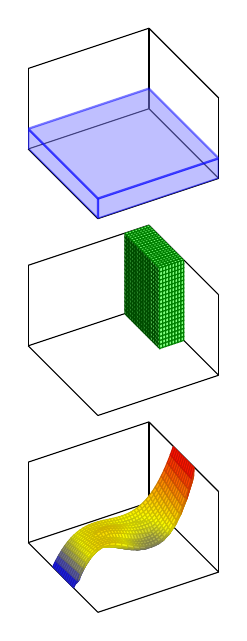
\begin{tikzpicture}

\begin{scope}[shift={(0,4)}]
\begin{axis}[
   width=4cm, height=4cm,
   xmin=0, xmax=1,
   ymin=0, ymax=1,
   zmin=0, zmax=1,
   view={-30}{45},
   xtick=\empty, ytick=\empty, ztick=\empty,
   ]
   % draw lower box
   % front
   \draw[thick,blue,fill=blue!50,opacity=0.5]
      (axis cs:0,0,0) -- (axis cs:0,0,0.25) -- (axis cs:1,0,0.25) -- (axis cs:1,0,0.0) -- cycle;
   % side (left)
   \draw[thick,blue,fill=blue!50,opacity=0.5]
      (axis cs:0,0,0) -- (axis cs:0,0,0.25) -- (axis cs:0,1,0.25) -- (axis cs:0,1,0.0) -- cycle;
   % top
   \draw[thick,blue,fill=blue!50,opacity=0.5]
      (axis cs:0,0,0.25) -- (axis cs:1,0,0.25) -- (axis cs:1,1,0.25) -- (axis cs:0,1,0.25) -- cycle;
\end{axis}
\end{scope}

\begin{scope}[shift={(0,1.5)}]
\begin{axis}[
   width=4cm, height=4cm,
   xmin=0, xmax=1,
   ymin=0, ymax=1,
   zmin=0, zmax=1,
   view={-30}{45},
   xtick=\empty, ytick=\empty, ztick=\empty,
   ]
   % RxRE side surface (domain is z)
   \addplot3[
      surf,green!50!white,faceted color=green!30!black,
      samples=21,samples y=21,
      domain=0:1,y domain=0.5:1.0,
      z buffer=sort]
      ({0.8}, {y}, {x});
   % RxRE front surface (domain is z)
   \addplot3[
      surf,green!50!white,faceted color=green!50!black,
      samples=21,samples y=9,
      domain=0:1,y domain=0.8:1.0,
      z buffer=sort]
      ({y}, {0.5}, {x});
   % top front surface
   \addplot3[
      surf,green!50!white,faceted color=green!50!black,
      samples=9,samples y=21,
      domain=0.8:1,y domain=0.5:1.0,
      z buffer=sort]
      ({x}, {y}, {1.0});
\end{axis}
\end{scope}


\begin{scope}[shift={(0,-1)}]
\begin{axis}[
   width=4cm, height=4cm,
   xmin=0, xmax=1,
   ymin=0, ymax=1,
   zmin=0, zmax=1,
   view={-30}{45},
   xtick=\empty, ytick=\empty, ztick=\empty,
   ]
   % bottom of RxO (front, negative y half only)
   \addplot3[
           surf,
           opacity = 1.0,
           samples=21,
           samples y=21,
           domain=0:1,y domain=-1:0,
           z buffer=sort]
       ({x},
        {(0.5+0.15*(y))},
        {max(0.0, ((8*x^3 - 11*x^2 + 4*x)*(1-(0.5+0.15*(y))^2) + (x)*((0.5+0.15*(y))^2))
           - (0.1 + 0.04*abs(24*x^2 -22*x + 4))*max(0.00001,(1-y^2))^0.5)});
   % top of RxO (negative y half)
   \addplot3[
           surf,
           opacity = 1.0,
           samples=41,
           samples y=13,
           domain=0:1,y domain=-1:1,
           z buffer=sort]
       ({x},
        {(0.5+0.15*(y))},
        {((8*x^3 - 11*x^2 + 4*x)*(1-(0.5+0.15*(y))^2) + (x)*((0.5+0.15*(y))^2)) + 0.05*(max(0.00001,1-(2*y)^2-2*(3*(x-0.5))^2))^0.5});
\end{axis}
\end{scope}

\end{tikzpicture}
\end{document}
